\chapter{Semantic Tags for Open Data Portals}
\label{chap:tagging}


As observed in the previous chapter, literature related to semantic enhancement of ODPs metadata has still some significant gaps, such as:
\begin{itemize}
	\item Emerging semantics from the ODP context;
	\item Dealing with multiple languages;
	\item Tags attributed by few users, in a non-folksonomy style;
	\item Integrating multiple domains.
\end{itemize}

In order to	tackle this issue, we describe in this chapter the Semantic Tags for Open Data Portals - STODaP approach for improving tag curation within and across ODPs, and for linking ODPs through its metadata.

Besides the comprehensive analysis of tag usage in 87 ODPs, shown in previous chapter, that justifies the need and benefits of better tools for managing tags, our main contributions are:
\begin{itemize}
	\item An approach for cleaning and reconciliation of metadata in ODPs;
	\item An approach for semantic lifting of metadata in ODPs;
	\item A centralized repository for connecting ODPs through meaningful shared tags.
\end{itemize}

This chapter begins with a short motivation to the topic of our work.
For a deeper analysis, readers are referred to the the previous chapters.
% In the first section, some considerations about metadata in open data portals are derived. 
% In the following, the different concepts of tagging are put into perspective, in order to characterize tags in ODPs. 
% \autoref{sec:analysis} presents an analysis of the use of tags in several Open Data Portals, both from government and civil society side, and from various countries and languages.
The main part of this chapter lies in \autoref{sec:stodap_architecture}, where our approach for semantic tags in open data portals is explained.
STODaP architecture is detailed, and every module and their connections is explained.
In the following, \autoref{sec:implementation} presents the implementation architecture, detailing the technological choices used to build the STODaP platform and the associated plugins.
We present afterwards some quantitative results in \autoref{sec:results}, and finish with a conclusion regarding the developments presented in this chapter.
An evaluation of the approach is driven in \autoref{chap:evaluation}.

%#########################################################################################
\section{Motivation}
%#########################################################################################

Analysing large amounts of data plays an increasingly important role in today's society. 
However, new discoveries and insights can only be attained by integrating information from dispersed sources. 
Despite recent advances in structured data publishing on the Web (such as RDFa and the schema.org initiative) the question arises how larger datasets can be published and described in order to make them easily discoverable and facilitate the integration as well as analysis.

One approach for addressing the problem of data dispersion are data catalogues, which enable organizations to upload and describe datasets using comprehensive metadata schemes. 
Similar to digital libraries, networks of such catalogues can support the description, archiving and discovery of datasets on the Web. 
Recently, we have seen a rapid growth of data catalogues being made available to the public. 
The data catalogue registry \href{http://datacatalogs.org}{datacatalogs.org}, for example, already lists 285 data catalogues worldwide. 

Data catalogues where data is supposed to be open, at least in the licensing sense, are usually called Open Data Portals (ODPs).
Implementations that show the increasing popularity of ODPs can be seen, for example, in open government data portals, data portals of international organizations and NGOs, as well as scientific data portals.

In order to increase transparency and citizen engagement, governments and public administrations all over the world are implementing ODPs. 
These ODPs comprise large amounts of structured data, mostly in the form of tabular data such as CSV files or Excel sheets. 
They aim to be a one-stop-shop for citizens and companies interested in using public data produced by governments or civil society organisations.
Examples are the \href{http://data.gov}{US' data portal}, the \href{http://data.gov.uk}{UK's data portal}, the \href{http://open-data.europa.eu}{European Commission's} portal as well as numerous other local, regional and national data portal initiatives.

In the research domain ODPs also play an important role.
Almost every researcher works with data. 
However, quite often only the results of analysing the data are published and archived. 
The original data, that is ground truth, is often not publicly available thus hindering repeatability, reuse as well as repurposing and consequently preventing science to be as efficient, transparent and effective as it could be. 
An example of a popular scientific open data portals is the \href{http://data.gbif.org}{Global Biodiversity Information Facility Data Portal}.
Also many international and non-governmental organizations operate ODPs such as the \href{http://data.worldbank.org}{World Bank Data Portal} or the data portal of the \href{http://apps.who.int/gho/data/}{World Health Organization}.
Although being a relatively new type of information system first commercial (e.g. Socrata) and open-source (e.g. CKAN) data portal implementations are already available.

% Despite its recent popularity, Open Data and Open Data Portals still face significant impediments, as richly described in \autoref{sec:problems}.
% Authors collected 118 socio-technical impediments for use of open data from interviews, workshops and literature.
% Some cited impediments were ``absence of commonly agreed metadata'', ``insufficiency of metadata'', ``the lack of interoperability'' and ``difficulty in searching and browsing data'', showing that a great challenge for ODPs is the organization of data.

% The open data organization challenge can be subdivided into two aspects: 1) structuring and organizing the datasets themselves and 2) providing well-structured and organized metadata for the datasets.
% The first aspect was, for example, tackled by approaches for semantic lifting of data by~\cite{DBLP:conf/i-semantics/ErmilovAS13} and~\cite{Ding2011325}, who tried to build general strategies for putting large open government datasets in the Link Data cloud.
% For the standardized structuring metadata, the Data Catalog Vocabulary (DCAT)\footnote{Available at \url{http://www.w3.org/TR/vocab-dcat/}}~\cite{conf/i-semantics/CyganiakMP10} was developed.
% However, the cross-portal metadata alignment and reconciliation can not be addressed by DCAT.

The metadata used to organize datasets in an ODP comprises categories or groups and most importantly labelling with free-text words or sets of words -- the tags.
The concept of tagging became popular within Web 2.0 services and aggregation tools like del.icio.us. 
The main advantages of tagging are the ease of classifying, and the crowd effect -- resulting in the so called folksonomies -- because all users are allowed to tag and share their contents. 
Tagging datasets in an ODP cannot be considered as folksonomies, because the process is mainly driven by portal managers and data publishers, and not by the actual users.
As a result of this, the structuring effect of crowd-tagging and folksonomies is missing in ODPs.

A quick look over some ODPs reveals that most of them suffer from a very confusing organization of datasets. 
The first level of categorization uses the concept of groups.
In general, they are stable and meaningful, but normally contain a large number of datasets.
A more detailed classification should be done via tags, whose use in ODPs has the following issues:

\begin{itemize}
	\item \emph{Synonyms:} In most ODPs, there exists large number of synonymous tags, e.g., \texttt{crops} and \texttt{seeds};
	\item \emph{Different spellings of the same word:} Several tags are incorrectly written, or have differences in capitalization or accents, e.g., \texttt{baden-wuerttemberg} and \texttt{Baden-W\"{u}rttemberg};
	\item \emph{Lack of relationships:} There is no explicit relationships between the tags, e.g., \texttt{Community Centres} is clearly a specialization of \texttt{Community}, but this is not explicit;
	\item \emph{Ambiguity:} As tags are written as pure text, ambiguity is prevalent in ODPs, e.g., the tag \texttt{apple}, which could refer to the fruit or to the company; and
	\item \emph{Incoherence:} Tags do not allow any connection between different portals that use the same or equivalent tags, e.g., two datasets tagged with \texttt{budget} in different portals are not connected.
\end{itemize}

As a result, the navigation, exploration and search within individual, but in particular also across ODPs is significantly hampered.
Thus, we present in the following the STODaP architecture, whose intention is to facilitate access to open data.


%#########################################################################################
\section{The STODaP Architecture}
\label{sec:stodap_architecture}
%#########################################################################################

In this section, we present the tag reconciliation approach for cleaning up and connecting ODPs, supported by software tools both at the local and global contexts.
The objective of this approach is to tackle the main problems identified by metrics described in \autoref{sec:analysis}, and thus to ease data organization and linking through metadata descriptions of ODPs.

\autoref{fig:overview}\footnote{Icons by \href{http://www.flaticon.com/authors/simpleicon}{SimpleIcon} from \href{http://www.flaticon.com}{www.flaticon.com} are licensed under \href{http://creativecommons.org/licenses/by/3.0/}{CC BY 3.0}.} shows an overview of the proposed approach.
Data publishers in charge of ODPs are offered tools for enhancing local tag curation and semantic lifting.
These local tags are then connected to semantic tags hosted in a central server, which is automatically fed by data coming from ODPs.
% They can add new semantic descriptions to the global tags, establish relations between them, and also create new links between global and local tags.
Data consumers have the option to retrieve data directly from ODPs, or through references gathered from the central server.
%The description of these actions is shown in the sequel.

\begin{figure*}[t]
\begin{center}
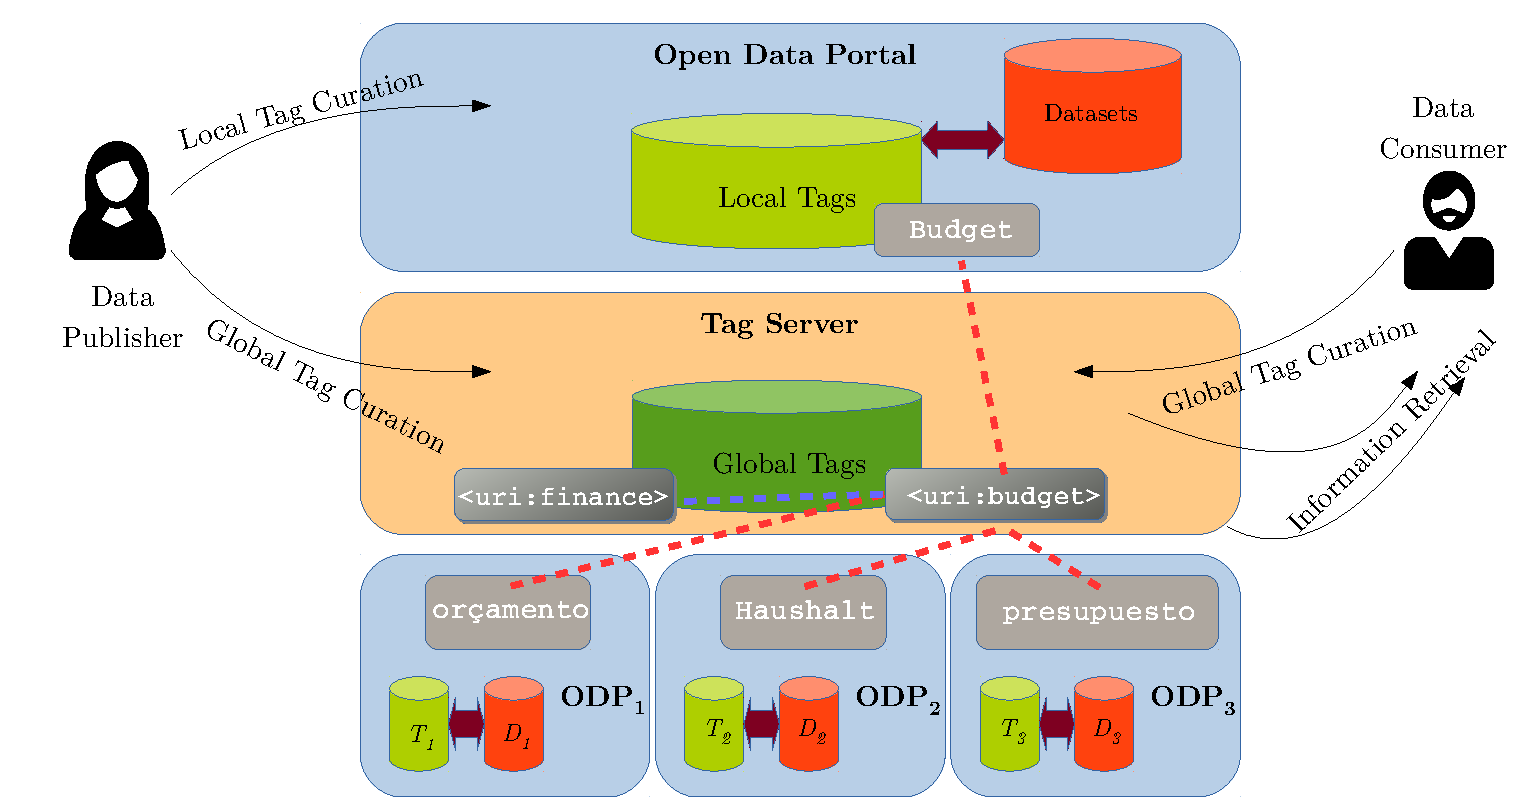
\includegraphics[width=\columnwidth]{images/overview.pdf}
\caption[Overview of the STODaP approach.]{Overview of the STODaP approach. Local tags are connected to a corresponding semantic tag within a central tag server. 
Data managers responsible for ODPs may use tools for local tag curation and semantic lifting of metadata.}
\label{fig:overview}
\end{center}
\end{figure*}

This section is divided as follows: first, we present an overview of the STODaP architecture in \autoref{sec:stodap_architecture_overview}.
The following subsections describe each element of this architecture, i.e., Open Data Portals (\autoref{sec:definition}), external plugins (\autoref{sec:tag_manager_plugin}), local and global Processing steps (\autoref{sec:local_building} and \autoref{sec:global_building}), Semantic Metadata Repository (\autoref{sec:semantic_metadata_repo}),  STODaP vocabulary (\autoref{sec:stodap_vocabulary}), and query interfaces.

% %#########################################################################################
\subsection{Architecture Overview}
\label{sec:stodap_architecture_overview}
% %#########################################################################################

\autoref{fig:architecture} depicts the architecture of STODaP approach.
The system receives as main input metadata of Open Data Portals, which are basically dataset descriptors such as title, description, tags, themes and others.
These metadata are individually pre-processed for each portal at the Local Processing phase, and stored at the Metadata Repository.
These metadata are individually pre-processed for each portal at the Local Processing phase, and stored at the Metadata Repository.
Metadata are also jointly processed, together with data coming from semantic knowledge bases from the Linked Open Data cloud, at the Global Processing phase.
This phase results in the Semantic Tags and Groups, which are then coded using the STODaP vocabulary.
Resultant dataset is made available for the general public through three types of interfaces: an HTML website where users can navigate manually, an RDF/XML interface which responds to machine requests searching for the URIs resources, and a SPARQL endpoint, which accepts queries and responds with JSON coded triples.
In addition, the STODaP approach also offer plugins for ODPs to enhance tag management and to link local tags with the server.
The STODaP approach is independent of these plugins, and their implementation is under control of ODP administrators.

\begin{figure*}[t]
\begin{center}
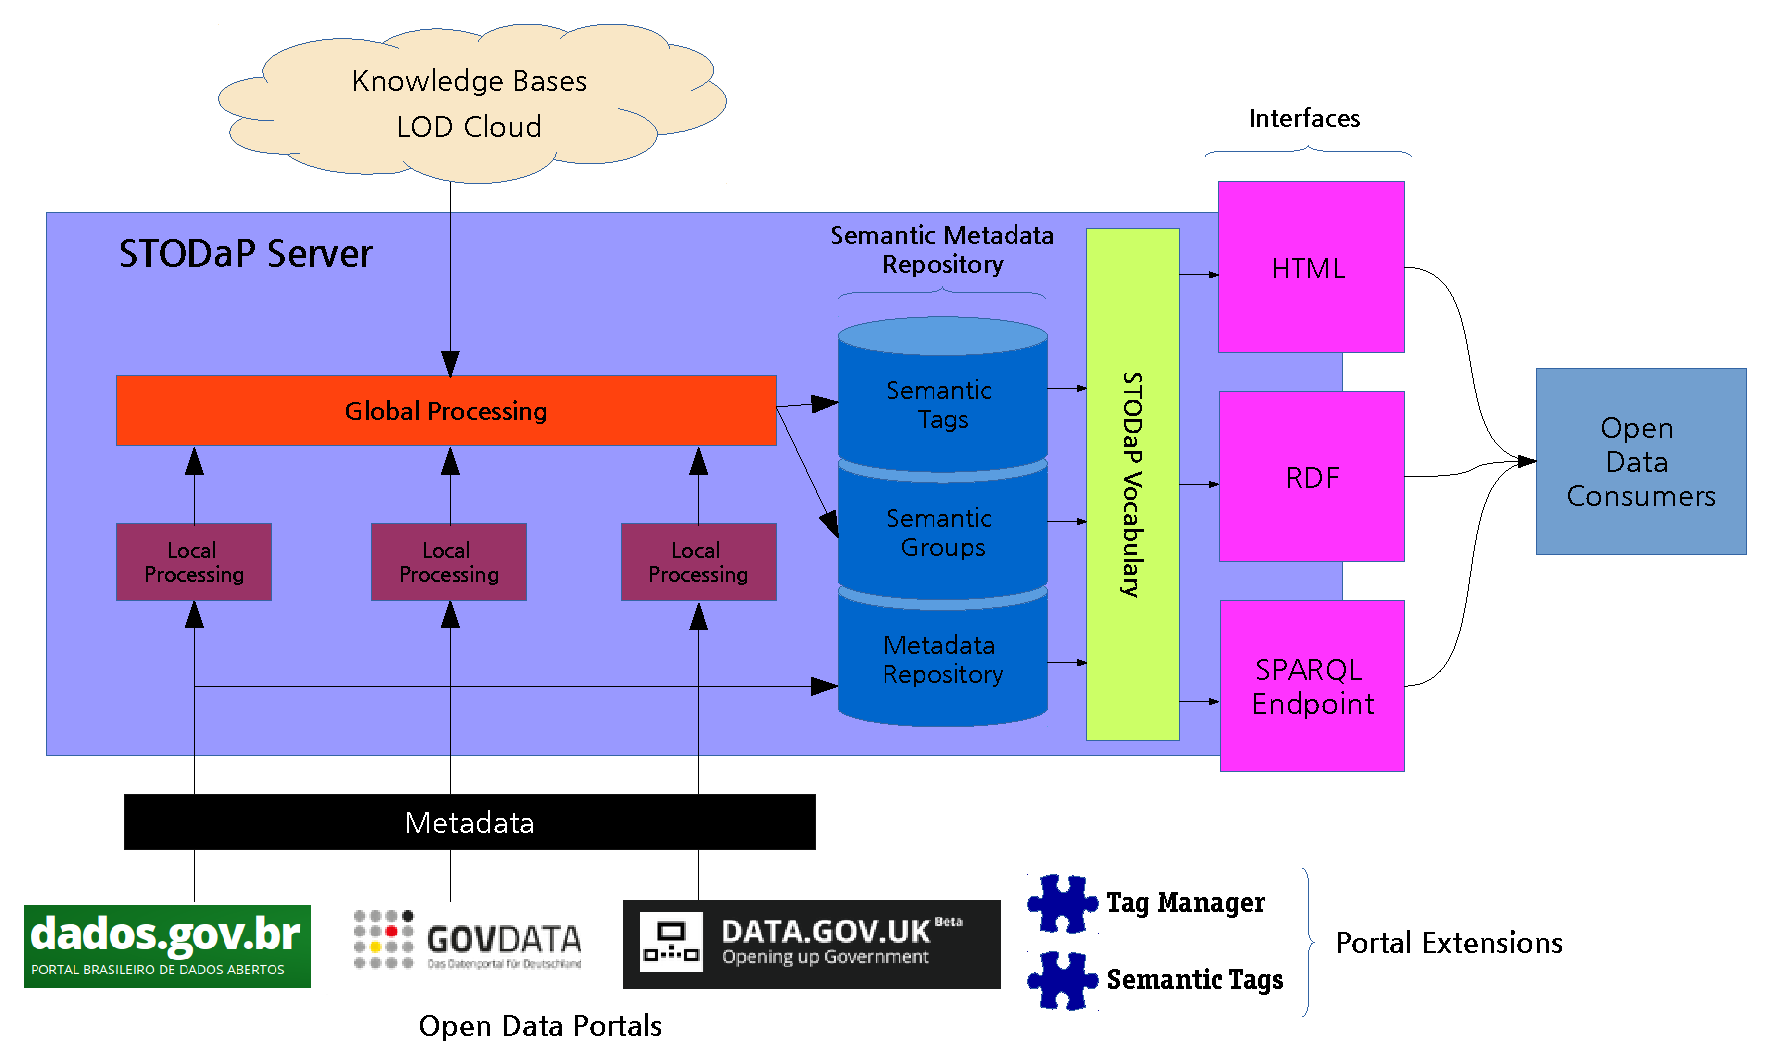
\includegraphics[width=\columnwidth]{images/architecture.pdf}
\caption[Architecture of the STODaP approach.]{Architecture of the STODaP approach.}
\label{fig:architecture}
\end{center}
\end{figure*}

In the following, each of these blocks is explained in details.

%#########################################################################################
\subsection{Open Data Portals}
\label{sec:definition} 
%#########################################################################################

\begin{figure}[t]
\begin{center}
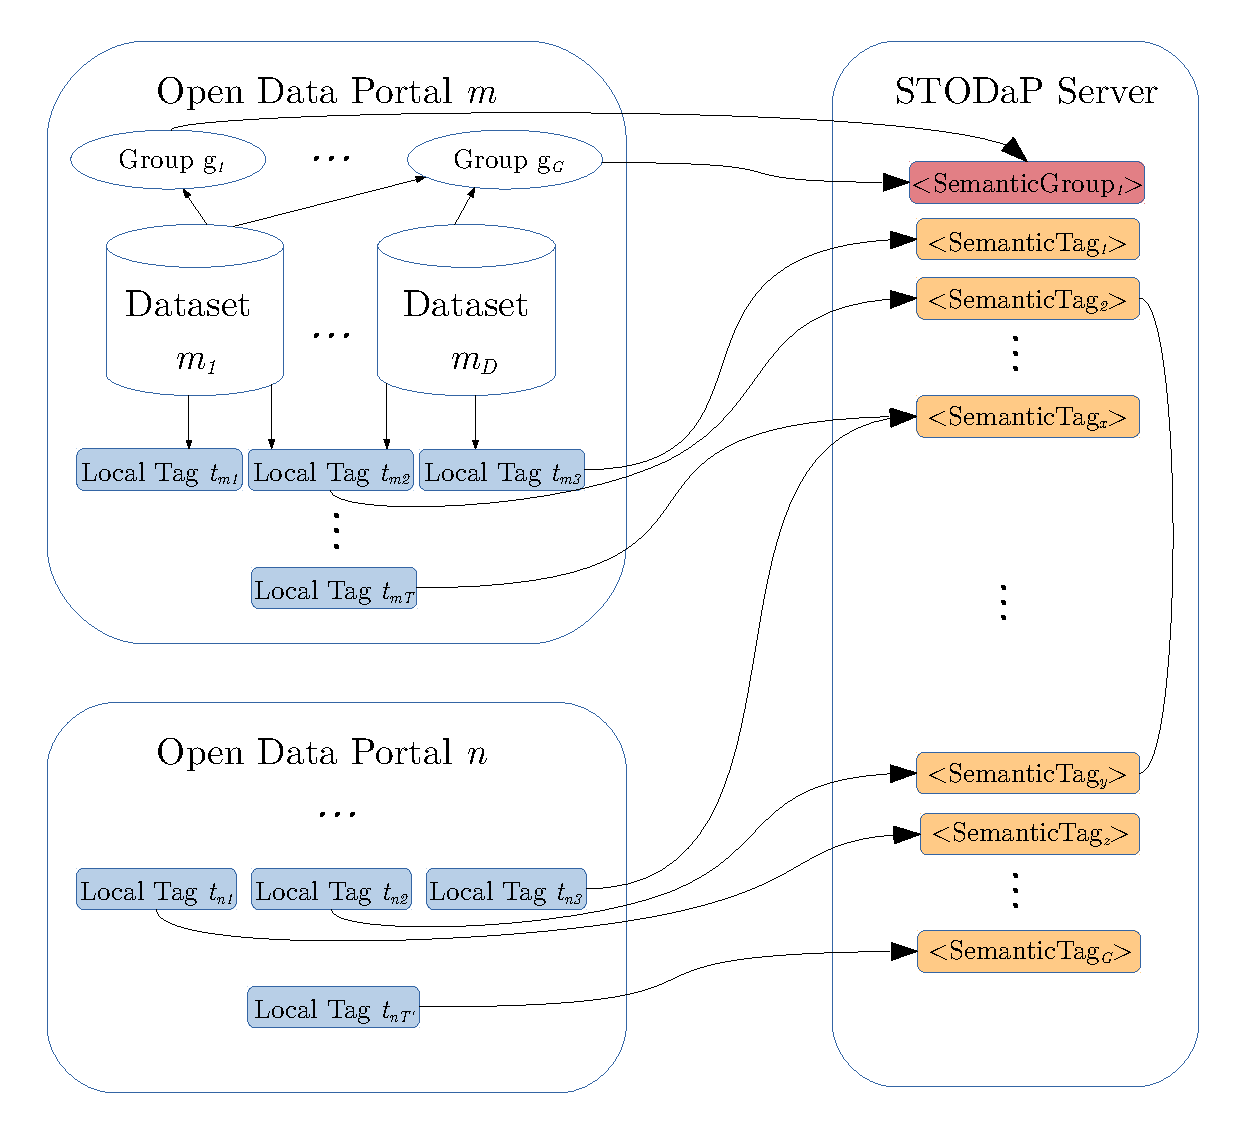
\includegraphics[width=\columnwidth]{images/odp_definition.pdf}
\caption{Relevant elements of the Semantic Tags for Open Data Portals system.}
\label{fig:definition}
\end{center}
\end{figure}

According to~\citeonline{Colpaert2013}, an Open Data Portal is ``a collection of systems set up to make Open Data used and useful''.
This definition sounds quite ambitious, since the great majority of ODPs are not a collection of systems, but of datasets.
A formal definition of an ODP can be found in~\citeonline{Umbrich2015}.
However, in that case, the focus is quite general and complex, which turns their definition unsuitable to be used here. 
In this section, we will describe the elements that are present in the context of this work.

\autoref{fig:definition} shows the relevant entities and relations that are present in ODPs and their relation to the STODaP server.
An \emph{Open Data Portal}, in this context, is a collection of datasets, which can be managed by governments, NGOs, universities or other institutions.
Open Data Portals are managed authorized users, who are in charge of uploading resources and filling metadata fields.

\emph{Datasets} are containers that can hold one or more open data resources of several formats, including csv, xls, json, and even non-open ones, such as pdf.
Most ODP metadata are associated to datasets, and the main ones are name, description, author, date, maintainer, and tags.

\emph{Groups} are dataset containers, and are used normally to organize datasets by theme. One group can hold several datasets, and one dataset can be associated to several groups (or none).

\emph{Tags} are a metadata element which is defined a string that represents its name.
Every distinct string represents a different tag, and every dataset tagged with tags represented by the same string can be sorted using this tag.
Tags normally refer to the specific theme dealt by the dataset.
However, it is quite frequent that tags represent temporal or geographical references.
It must be emphasized that tags, in this context, are not related to a tagger, i.e., the person who tags.
This happens in folksonomy contexts \cite{Grubber2007}, which, as previously discussed, is not our case.
A dataset can be tagged with several (or no) tags, and a tag can be related to one or more datasets.
At the CKAN platform, it is possible to have a tag not related to any dataset, however, we will not consider those ones.
In our context, we will define tags as \emph{Local Tags}, in order to emphasize that they only exist in a single ODP context.

In order to illustrate the whole architecture, we also show the connections between Tags and \emph{Semantic Tags}, and between Groups and \emph{Semantic Groups}.
Several local tags from different ODPs can be associated to a single semantic tag, which can also have semantic relationships with other semantic tags.

The STODaP architecture also includes plugins to enhance metadata inside ODPs.
Two of these add-ons will be presented in the following.
It is important to highlight that these plugins are external to the STODaP server, and can only be installed and used by ODP managers.

%############################################################
\subsection{Portal Extensions - Cleaning up and semantifying tags}
\label{sec:tag_manager_plugin}
%############################################################

\noindent\textbf{Tag Manager}

\autoref{sec:local_metrics} showed that ODPs suffer from low reuse of tags, and that there is a significant tags duplication due to slight spelling differences. 
In fact, both problems -- low reuse and duplication -- are connected, since merging similar tags improves tag reuse.
However, low tag reuse can be also attributed to the absence of a standard tagging procedure, which would guide users in this task.

To address this problem locally at a particular ODP, we propose an approach for clean-up and reconciliation of tags. %, and for enhancing the quality of the new ones.

First, we offer three levels of semi-automatic tag merging strategies:

% spell 
% check for sem similatyy libs in phyton

\begin{enumerate}
	\item With high confidence, we suggest merging tags that differ only by capital letters or special characters. 
In many ODPs, this strategy will already achieve significant results, as shown in \autoref{fig:similarity}.
	\item After running the first strategy, the Levenshtein distance is computed for all remaining pairs of tags.
Tags with distance one or two are suggested for merging, in order to catch plural/gender variations, such as \texttt{worker} and \texttt{workers}. 
However, false-positives like \texttt{widow} and \texttt{window} may appear.
Tags composed only by numbers (to avoid merging tags representing years) or less than 4 characters are not included.
	\item Finally, we use semantic measures~\cite{Harispe01032014} to determine the semantic similarity between two tags. 
In this case, the tags \texttt{autumn} and \texttt{fall} have a high similarity, and thus will be suggested for merging.
\end{enumerate}

%For the new tags, besides suggesting tags that were already used in the portal, we also suggest tags based on the previous tags (and on the context???). 
It must be noted that all these approaches have originally quadratic time complexity, because every pair of tags has to be computed. However, sorting tags alphabetically turns the problem into linear in strategies 1 and 2 (however, with possible losses in 2), and ignoring tags without correspondence in dictionary reduces the dimension in strategy 3.

\noindent\textbf{Semantic Tags}

After this cleaning procedure, we offer users the opportunity to link each local tag to a semantic correspondent at the tag server.
The main idea is to enable not only the connection between ODPs and the STODaP server, but also the other way around.
The semantic tags plugin automatically suggests connections between local tags and semantic tags.
Connections can also be done manually.

Linking local and semantic tags can bring several benefits for users navigating in ODPs, such as: better search options based on semantic tags; recommendation of similarly tagged datasets located in other portals; or taking advantage of the structure provided by the relationships between semantic tags, and consequentially, between local tags.

--

In order to build the first version of the STODaP server, a metadata harvesting was driven through 87 ODPs.
Almost 500.000 datasets were processed, including their metadata such as names, language, tags and groups they belong to.
In the following subsection, we describe the procedures applied to the individual portals, in the process called Local Processing, which refers to the fact that it deals only with individual ODPs data.


%##################################################################
\subsection{Local Processing - Clean Up and Reconcile}
\label{sec:local_building}
%##################################################################

The first processing step inside the STODaP server works over metadata of each ODP, and thus is called \emph{Local Processing}.
An overview of the procedure applied for each ODP is shown in \autoref{fig:local_processing}.
In the figure, each green block represents a processing phase, which is materialised in a set of tag representations. 
The grey blocks describe the transformations suffered by the tag sets from one phase to another.
The aim of the local processing steps is to transform freely written tags into semantic resources that are candidates for representing the datasets they are associated.
Each transformation applied to the tags on the local processing is detailed bellow:

\begin{figure*}[b]
\begin{center}
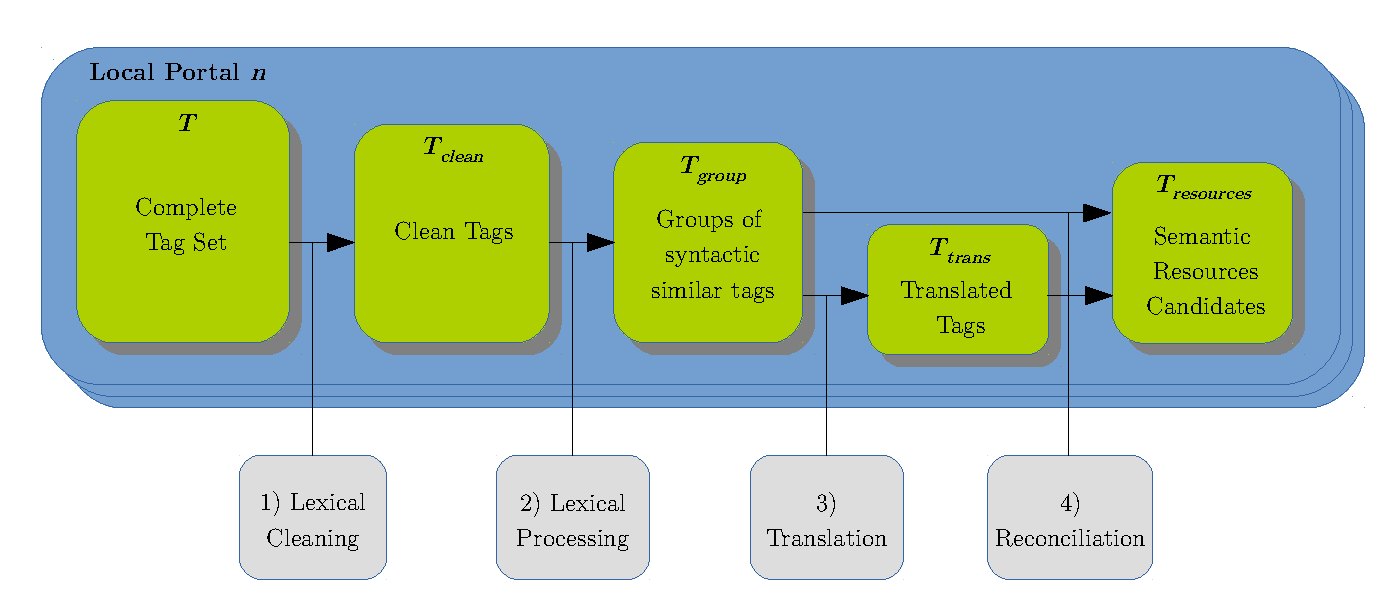
\includegraphics[width=\columnwidth]{images/local_processing.pdf}
\caption{Overview of the local tag processing.}
\label{fig:local_processing}
\end{center}
\end{figure*}

\noindent \textbf{Lexical Cleaning: }The complete tag set $T$ is the set containing all original tags found in one portal.
Firstly, the \emph{Lexical Cleaning} is applied in order to discard tags with low probability of getting a semantic meaning.
At this point, some heuristics are applied, and a tag is discarded if it is: 
\begin{itemize}
	\item smaller than 4 characters; 
	\item composed of numbers and alphabetic characters;
	\item exclusively composed by uppercase characters;
	\item not started by a alphanumerical character;
	\item larger than 5 words; or
	\item not applied to any dataset.
\end{itemize}

\noindent \textbf{Lexical Processing:} After the Lexical Cleaning, we have the resulting set $T_{clean}$ of clean tags, with a higher probability of being reconciled with semantic concepts in ontologies.
The following procedure is the \emph{Lexical Processing}, which aims to group tags that have a lexical similarity.
These similar tags have a high probability of representing the same meaning, with small lexical variations.
In order to determine this similarity, we apply the Levenshtein edit-distance to the lowercased and unaccented tags (which means that \texttt{Açaí} will be transformed into \texttt{acai} before measuring the distance).
Based on manual experimentation, we consider that tags with an edit-distance of 0 or 1 are similar.
This distance captures plural, gender and temporal variations in most of the languages present in our sample.
The proceeding results in the set $T_{group}$ of syntactically similar tags.

\noindent \textbf{Translation:} The sample used to build this tag server contains portals in 22 different languages.
Thus, it is necessary to use translation services on the Web to transform words from their original language to the English language.
English language was chosen because of the higher availability of translation services, and also because the main ontologies have their terms described necessarily in English, and possibly also in other languages.
It also significant that 43\% of the portals are in English (according to the provided metadata), and their tags represent 83\% of all tags.
Each group of similar tags from $T_{group}$ was translated, resulting possibly in a set of translations for each group.
The new set achieved in this processing is $T_{trans}$.

\noindent \textbf{Reconciliation:} The previous proceeding results in a set $T_{trans}$ of groups formed by all the related translations.
Until this moment, we were dealing with string of characters.
In this stage, these names will be the input for searching semantic representations for the tags.
In order to get the widest spectrum of possibilities, the search for semantic resources is done for all lexical representations of the tag, stored in $T_{group}$, and also all possible translations of it in $T_{trans}$.
The resulting set will be denominated $T_{resources}$.

%The product of this step are synonym rings, or synsets, where the groups of words have are semantically equivalent for the purpose of retrieving information.
%The proceeding results in the set $T_{synt\_sem}$ of semantically similar tags.

%Finally, in order to prepare the tags for linking with other portals, we come to the \emph{Translation} step.
%Each tag is translated to the English language, forming the set $T_{english}$ of translated tags.
%->> tentar todas as opções de tradução
In order to illustrate the procedure, \autoref{tab:local_example} shows an example using real tags from the Brazilian Data.gov.br.
From $T$ to $T_{clean}$, tags containing numbers, too small or representing abbreviations were removed.
Then, similar tags were grouped to form $T_{group}$.
The translation process could not find an equivalent for the first group.
Even so, the semantic search-engine was able to find a matching resource for \texttt{Acidente de trabalho} (accident at work), as well as for the other two.

\begin{table}[]
\centering
\ABNTEXfontereduzida
\caption{Examples of tags in each step of the procedure.}
\label{tab:local_example}
\begin{tabular}{|p{2cm}|p{2cm}|p{2cm}|p{2cm}|p{2cm}|p{2cm}|}
\hline
$T$ & $T_{clean}$ & $T_{group}$ & $T_{trans}$ & $T_{resources}$ \\ \hline
Acidente de trabalho,
Acidentes de trabalho,
CNAE,
finanças,
Folha SA.23,
Folha SB.23 
município,
orçamento,
UF
&
Acidente de trabalho,
Acidentes de trabalho,
finanças,
orçamento
&
\{Acidente de trabalho, Acidentes de trabalho\}
finanças,
orçamento
&
--
finances,
budget
&
\{gemet:9366, eurovoc:825\},
eionet:3194
eionet:1025 \\ \hline
\end{tabular}
\end{table}

It is important to notice that the process described above is subject to several failures.
On the Lexical Cleaning step, meaningful tags with less than 4 characters may be discarded, as well as unintentionally uppercased words.
On the Lexical Processing stage, it is possible that in some languages the same word starting with capital and non-capital letters have different meanings.
With a higher probability, words differing from edit-distance of 2 may also have different (or even opposed) meanings, such as \texttt{child-death} and \texttt{child-health}, found on data.gov.uk.
On the Translation phase, the main problem lies on polysemy, where the same word has several meanings.
While also heavily dependent on the translation tools, providing side tags or other metadata can help the algorithm finding the right translation.
Finally, when searching for the meanings, there is a great dependency on the tool used and the available knowledge bases.

%#######################################################################
\subsection{Global Processing - Interlinking Portals}
\label{sec:global_building}
%#######################################################################

After reaching the last stage of the local processing stage for each one of the 87 portals, a joint process starts over $T_{resources}$ in order to build the Semantic Tag Server.
At the global processing stage, there are three main steps:

\begin{enumerate}
	\item Select meaningful tags;
	\item Create semantic tags and connect local tags to them; and
	\item Discover and qualify relations between tags.
\end{enumerate}

In order to accomplish this objective, we propose the global procedure shown in \autoref{fig:global_processing}.

\begin{figure*}[tb]
\begin{center}
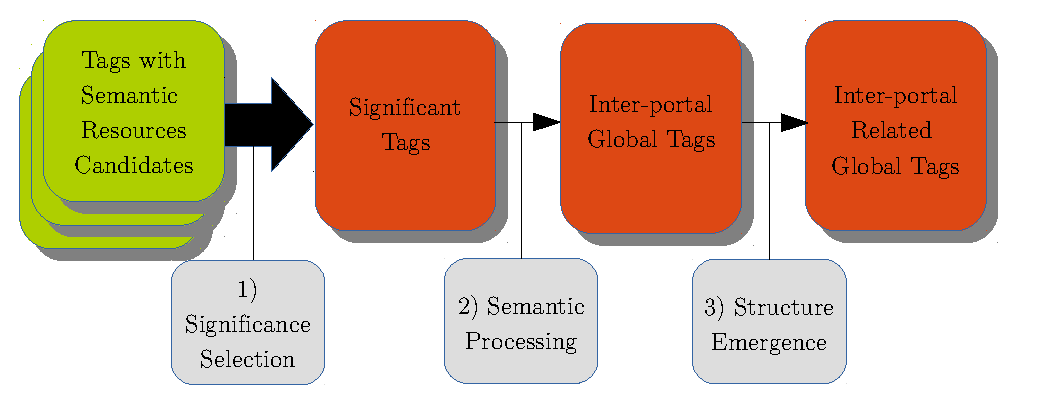
\includegraphics[width=\columnwidth]{images/global_processing.pdf}
\caption[Overview of the global processing.]{Overview of the global processing.}
\label{fig:global_processing}
\end{center}
\end{figure*}

\noindent \textbf{Significance Selection: } We start the global processing with a joint set $\mathcal{T}_{resources}$, which contains $T_{resources}$ from all portals. 
In this set, a \emph{Significance Selection} process is driven, in order to determine tags that will be useful on the information retrieval process.
This is an heuristics based process, which considers: (i) Success on finding semantic candidates for the tag; (ii) the number of datasets pointed by this tags; (iii) the quality of the semantic resources candidates.

\noindent \textbf{Semantic Processing:} After this step, the Semantic Tags will be derived.
Semantic Tags are entities on the web, who have a main name in English, several translations, and point to local tags, which in turn connect to datasets located into Open Data Portals.

\noindent \textbf{Structure Emergence:} Finally, relations between Semantic Tags in set $G$ will be searched on the ontologies they appear in order give a structure to the Semantic Tag set $G_{struct}$.
The first strategy is to search for relations on the reconciled ontologies, and set this relation between the semantic tags.
Thus, relations as \texttt{skos:related}, \texttt{skos:narrower} and \texttt{skos:broader} can be set.
However, at this point we notice need of an upper classification scheme.

The ODP model, as shown in \autoref{fig:definition}, includes a Group element, to which one or more datasets can be associated.
Thus, it is possible to consider that a tag associated to a dataset which is in a group is also related to this group.
However, only 11\% of all datasets in our sample are associated to groups, and only 13\% of the tags are associated to datasets in groups.

If we look to some ODPs which are organized in groups, it is possible to see a similar organization.
In \autoref{tab:groups}, we list the groups of 4 ODPs. 
If we look at the table, it is clear that in the context of open government data portals, there are some specific categories, but the portals also share common subjects, such as Health, Education or Culture.

\begin{table}[]
\centering
\ABNTEXfontereduzida
\caption{Examples of groups in some ODPs}
\label{tab:groups}
\begin{tabular}{|p{3.2cm}|p{3.2cm}|p{3.2cm}|p{3.4cm}|}
\hline
Data.gov & Data.gov.de & Dados.gov.br & Data.buenosaires.gob.ar \\ \hline
Aging / Agriculture / Business / Climate / Consumer / Disasters / Ecosystems / Education / Energy / Finance / Health / Law / Local Government / Manufacturing / Ocean / Public Safety / Science \& Research &
Population / Education and science / Geography, Geology and the GEODATA / Laws and justice / Health / Infrastructure, building and housing / Culture, leisure, sport, tourism / Not yet categorized / Public administration, budget and taxes / Politics and elections / Social / Transport and traffic / Environment and the climate / Consumer protection / Economy and work &
Municipal Chamber
/ trade, services and tourism
/ culture, leisure and sport
/ data sets in the spotlight
/ defence and security
/ economy and finance
/ education
/ public facilities
/ geography
/ government and politics
/ housing, sanitation and urbanism
/ health information
/ industry
/ justice and law
/ environment
/ person, family and society
/ management platform indicators
/ multi-year plan
/ international relations
/ health
/ work
/ transportation and transit &
economic activity /
public administration and policy /
culture and recreation /
education /
infrastructure and public works /
environment /
mobility and transport /
health and social services /
security /
urbanism and territory \\\hline
\end{tabular}
\end{table}

Thus, after translating all the group names, we verified that 62 group names occurred in three or more portals.
These were chosen as the first Global Groups.
The second step consisted in verifying the lexical similarity between all groups and the Global Groups in order to associate groups with Global Groups.
Some distortions were observed, such as \texttt{sport} being associated with \texttt{transport}, or \texttt{culture} with \texttt{agriculture}.
These errors were manually corrected.

Finally, groups were reconciled with general-purpose ontologies.
Particularly, the Gemet Thesaurus\footnote{Available at \url{http://www.eionet.europa.eu/gemet/}} fits well for this purpose.

%All Datasets: 470551
%Datasets in Groups: 53158
%Tags in Groups: 37743

%#######################################################################
\subsection{Semantic Metadata Repository}
\label{sec:semantic_metadata_repo}
%#######################################################################

After the Global Processing steps, Semantic Tags and Groups are ready to be stored at the \emph{Semantic Metadata Repository}, together with metadata originally collected from ODPs.

% With the aim of building a common basis for interlinking ODPs, we developed a Semantic Metadata Server.
% The conceptual rationale is:
% \begin{enumerate}
% 	\item To assist individual ODPs enhancing the quality of their tags, by assigning a common agreed meaning to them;
% 	\item To create a collaborative platform for meaningfully linking ODPs.
% \end{enumerate}

% The Semantic Metadata Server hosts the description of semantic tags and groups.
% Each semantic tag may be associated to one or more Linked Open Data resources, representing their semantic meanings.
% Linking to the local tags is accomplished via the URIs which represent a local tag in its context.
% The semantic tags can also have several types of relations between each other, such as \texttt{skos:broader}, \texttt{skos:narrower} or \texttt{owl:sameAs}.
% Figure \ref{fig:example} illustrates the concept with an example.

% \begin{figure}[tb]
% \begin{center}
% 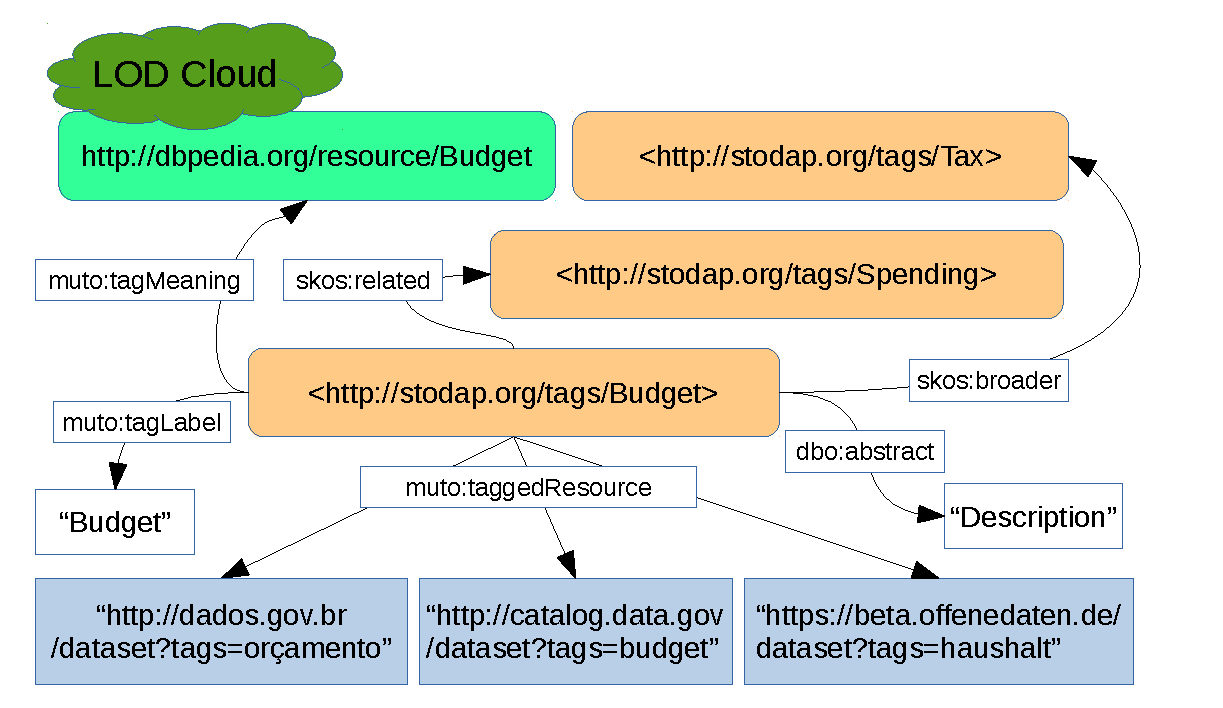
\includegraphics[width=\columnwidth]{images/example.pdf}
% \caption[Example of the STODaP model.]{Example of the STODaP model showing relationships of the semantic tag \url{http://stodap.org/tags/Budget}.}
% \label{fig:example}
% \end{center}
% \end{figure}

% The example shows the semantic tag identified by the URI \texttt{<http://stodap.org/tags/Budget>}. 
% With this semantic tag, a meaning and some URIs of local tags are associated.
% The semantic tag is also semantically related to other semantic tags, using the SKOS vocabulary.
% The MUTO ontology\footnote{\url{http://muto.socialtagging.org/core/v1.html}} is used to define some concepts and relations between the tags, like \texttt{muto:Tag}, \texttt{muto:taggedResource}, \texttt{muto:hasTag} and \texttt{muto:hasMeaning}.

%#######################################################################
\subsection{STODaP Vocabulary}
\label{sec:stodap_vocabulary}
%#######################################################################

\begin{figure*}[b]
\begin{center}
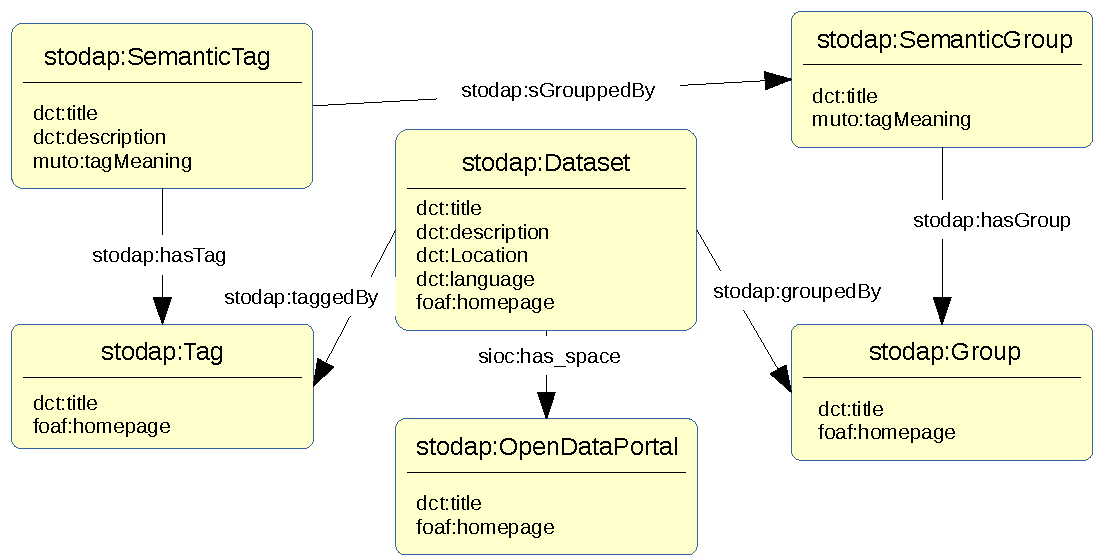
\includegraphics[width=\columnwidth]{images/stodap_vocabulary.pdf}
\caption[Simplified schema of the STODaP vocabulary.]{Simplified schema of the STODaP vocabulary. Some elements are equivalent to other vocabularies and ontologies, such as SIOC, DCAT and MUTO.}
\label{fig:vocabulary}
\end{center}
\end{figure*}

In order to represent data in our system, it was necessary to create a simple vocabulary.
\autoref{fig:vocabulary} shows a simplified schema of the STODaP vocabulary.
As shown in \autoref{sec:semantic_metadata}, several works describe ontologies and vocabularies related to our work.
However, it was not possible to fit all entities of STODaP architecture on existing ontologies.
Specifically, DCAT\footnote{Available at \url{http://www.w3.org/ns/dcat}.} defines some important entities, such as \texttt{dcat:Dataset} and \texttt{dcat:Catalog}.
They are defined as equivalent (\texttt{owl:equivalentClass}) to \texttt{stodap:Dataset} and \texttt{dcat:Catalog}, respectively.
At DCAT, tags are represented as literals, which means that two tags with the same label do not differ.
This is not the case at STODaP, where each tag is an entity.
MUTO\footnote{Available at \url{http://muto.socialtagging.org/}.} tackles this issue with the class \texttt{muto:Tag}, equivalent to our \texttt{stodap:Tag}.
On the semantic side, MUTO systematized the relation between a tag and a meaning with the \texttt{muto:tagMeaning} property.
Thus, although some concepts were reused, \texttt{stodap:SemanticTag} and \texttt{stodap:SemanticGroup} needed to be defined.
It must also be noted that MUTO works with a social concept of tagging, and thus defines a \texttt{muto:Tagging} class to enable relating actor to a tagging event, as described by~\citeonline{Grubber2007}.
Since the Open Government Data domain is not social, at least in the sense of tagging, this was not necessary in our case.

\noindent \textbf{\texttt{stodap:SemanticTag}:} A Semantic Tag is a super tag that groups open data portal tags and is connected to a semantic resource on the Linked Open Data Cloud.

\noindent \textbf{\texttt{stodap:SemanticGroup}:} A stodap:SemanticGroup is a super group of tags that groups open data portal groups, open data portal tags, and semantic tags. It is connected to a semantic resource on the Linked Open Data Cloud.

%#########################################################################################
\subsection{Interfaces}
\label{sec:interfaces}
%#########################################################################################

The last module of the STODaP architecture presented here is the Interfaces Modules.
Items in this module are designed to make data provided by the STODaP Server available for the external audience.

In order to respond to the various kinds of actors interacting with the STODaP server, 3 types of interface were designed.

\noindent\textbf{HTML - Human browsable interface}

The first interface is designed to offer ODP information for humans accessing the STODaP server.
This interface offers several options for users willing to find open datasets.
One option is to navigate through Semantic Tags.
Each Semantic Tag points to related local tags, which in turn are linked to tagged datasets.
Users are also presented related Semantics Tags (broader, narrower or related).
Following the same reasoning, it also possible to navigate though Semantic Groups an their related Semantic Tags, Groups and datasets.

Besides the navigation, the system also offers a keyword search interface.
In order to take advantage of the metadata organization system, a faceted search was designed.
Search is made in two steps: (i) user inserts a keyword; (ii) resulting datasets are presented, and may be filtered by 5 different facets: (a) Semantic Tags (b) Semantic Groups (c) Language (d) ODP (e) Country. 

\noindent\textbf{RDF - Dereferenceable URIs}

In order to be compatible with the fourth star of open data \cite{Berners-Lee2010}, each element of the STODaP server - Semantic Tags, Semantic Groups, Tags, Groups, Datasets and Open Data Portals have their own Unique Resource Identifier (URI).
This URI is also valid as URL, and accessed via the RDF interface, which responds with an RDF document containing the attributes of the referred element.

\noindent\textbf{SPARQL Endpoint}

The SPARQL endpoint provides direct access to the information stored in the Semantic Metadata Repository coded with the STODaP vocabulary.
Queries might be manually inserted, but can also be input via an API.
This requirement is important in order enable this repository to be link to automatic SPARQL queries generators, such as ...

%#########################################################################################
\section{Implementation}
\label{sec:implementation}
%#########################################################################################

In this section, we detail the technical choices related to the implementation of some elements of architecture presented in the previous section.
We start with an overview about the implementation of the STODaP server, detailing the software tools and integration strategies used, in \autoref{sec:implem_semtagserver}.
% In the sequence (\ref{sec:implem_semtags}), we give also details on the procedure for discovering the Semantic Tags discussed in \autoref{sec:global_building}.
A specific subsection is dedicated to the interface implementation, in \autoref{sec:implem_interface}.
Finally, we describe the implementation of two CKAN plugins in \autoref{sec:implem_plugins}:
(i) \emph{CKAN Tag Manager} and 
(ii) \emph{CKAN Semantic Tags}, which materialize the ideas reported in \autoref{sec:tag_manager_plugin}.

\subsection{Semantic Tags Server}
\label{sec:implem_semtagserver}

\begin{figure}[hb]
\begin{center}
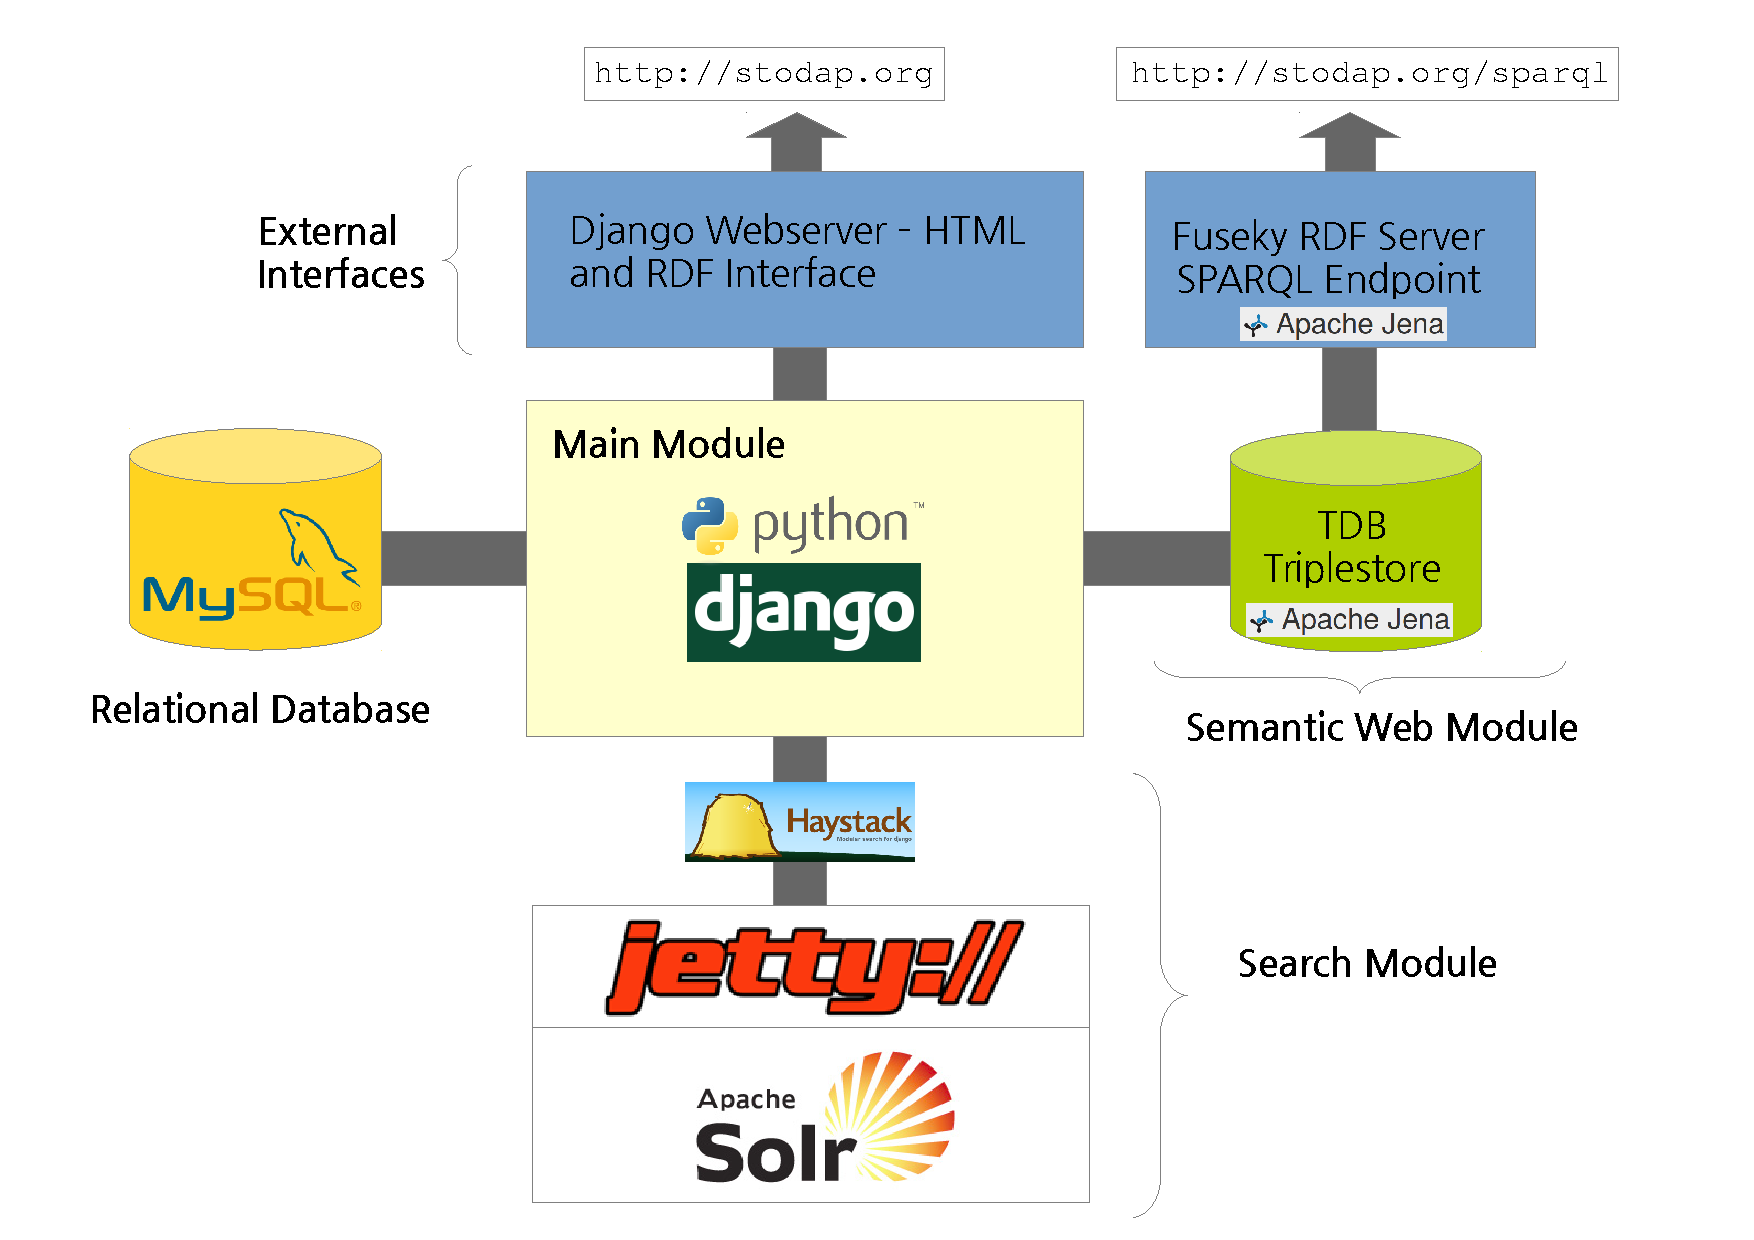
\includegraphics[width=\columnwidth]{images/implementation_architecture.pdf}
\caption[Implementation Architecture of the STODaP approach.]{Implementation Architecture of the STODaP approach.}
\label{fig:implem_arch}
\end{center}
\end{figure}

The first version of the STODaP server, presented in \citeonline{Tygel2016}, was implemented using \emph{MediaWiki} and specially the \emph{Semantic MediaWiki} extension~\cite{Kroetzsch2007}.
This extension turns the Wiki tool into a Semantic repository, facilitating the integration of objects into the Linked Open Data Cloud.

A second version of the STODaP server was developed, and the need of a more complete search platform, not present in MediaWiki was a main priority.
Thus, the most appropriate technological choice was to build an interface from scratch, integrated with a dataset that could be indexed by a search platform.
The implementation architecture can be seen in \autoref{fig:implem_arch}.

As core framework, STODaP uses the Django framework for Python Language.
This framework offers a rapid prototyping environment, with database integration and a web server for development purposes.
We integrated Django with a MySQL server, where the semantic metadata repository is stored in a relational database.

This database is indexed using Haystack Django plugin, which connects Django with an Apache Solr search platform.
Searching design option such as weights, facets and keyword logics are defined in Django and transformed into an XML configuration file which is used by Solr.
After this definition, Solr starts the indexing process, which enables the search mechanism.

In order to generate RDF triples, an Django2RDF converter was developed, based on the STODaP vocabulary.
The converter reads Django models and generates RDF files for each class: Dataset, Tag, Group, Semantic Tag, Semantic Group and Open Data Portal.
These files are upload into TDB Triplestore, which connects to the Fuseki RDF Server enabling a SPARQL endpoint.

% \subsection{Creating Semantic Tags}
% \label{sec:implem_semtags}

% \begin{itemize}
% 	\item Harvest all tags from portals
% 	\item Filter significant tags
% 	\item Group syntactically similar
% 	\item Translate - lexvo + yandex
% 	\item Reconcile - lexvo - several ontologies
% 	\item Choose gemet tags and create semantic tags and links
% 	\item Create global groups, and reconcile
% 	\item Associate semantic tags to global groups

	
% \end{itemize}

\subsection{Interfaces}
\label{sec:implem_interface}

Interfaces were implemented using Django Template language, which mixes HTML and a template syntax which allows basic logic operation (loops and conditions) and access to variables passed by the system.
CSS and Javascript were also used to build the screens.

\autoref{fig:stodap_welcome} shows the STODaP welcome screen.
An introductory text is presented, and is illustrated by a simplified STODaP model.
Some Semantic Tags and Groups are shown in order to motivate visitors.

An alphabetically ordered list of Semantic Tags is shown in \autoref{fig:stodap_semantictags}, and a specific Semantic Tag page can be seen in \autoref{fig:stodap_semantictag}.
Tha facet search interface is presented in \autoref{fig:stodap_search}
The complete system can be accessed at \url{http://stodap.org}.

\begin{figure}[h]
\begin{center}
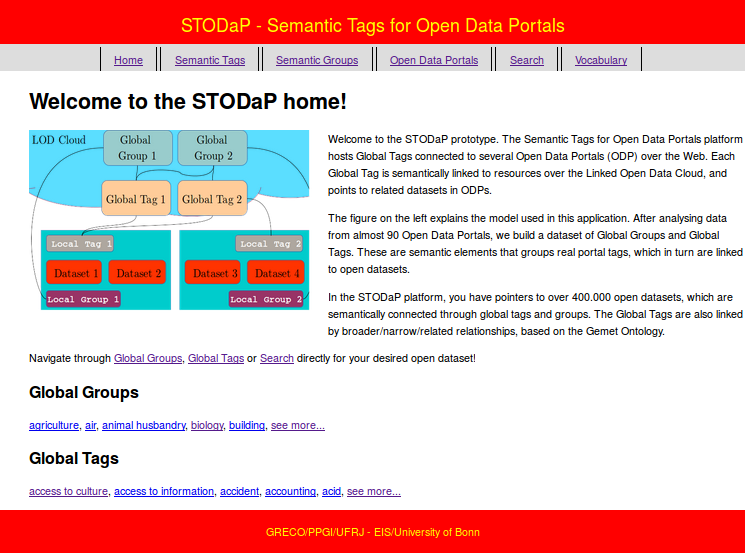
\includegraphics[width=\columnwidth]{images/stodapscreen_welcome.png}
\caption[STODaP welcome screen.]{STODaP welcome screen. An introduction text is presented, with a diagram showing the STODaP model. Some Semantic Tags and Groups are also displayed in order to motivate visitors.}
\label{fig:stodap_welcome}
\end{center}
\end{figure}

\begin{figure}[h]
\begin{center}
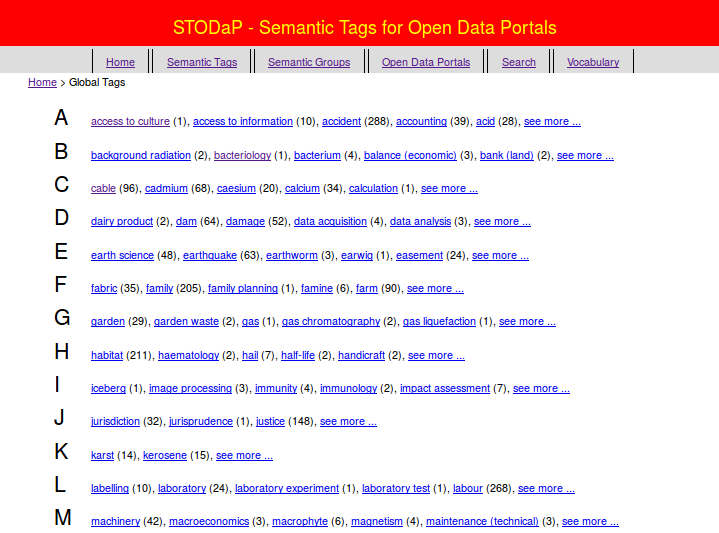
\includegraphics[width=\columnwidth]{images/stodapscreen_semantictags.png}
\caption[STODaP Semantic Tags.]{STODaP Semantic Tags. An alphabetically organized list is presented, in order to enable user navigation. In brackets, the number of datasets related to each tag.}
\label{fig:stodap_semantictags}
\end{center}
\end{figure}

\begin{figure}[h]
\begin{center}
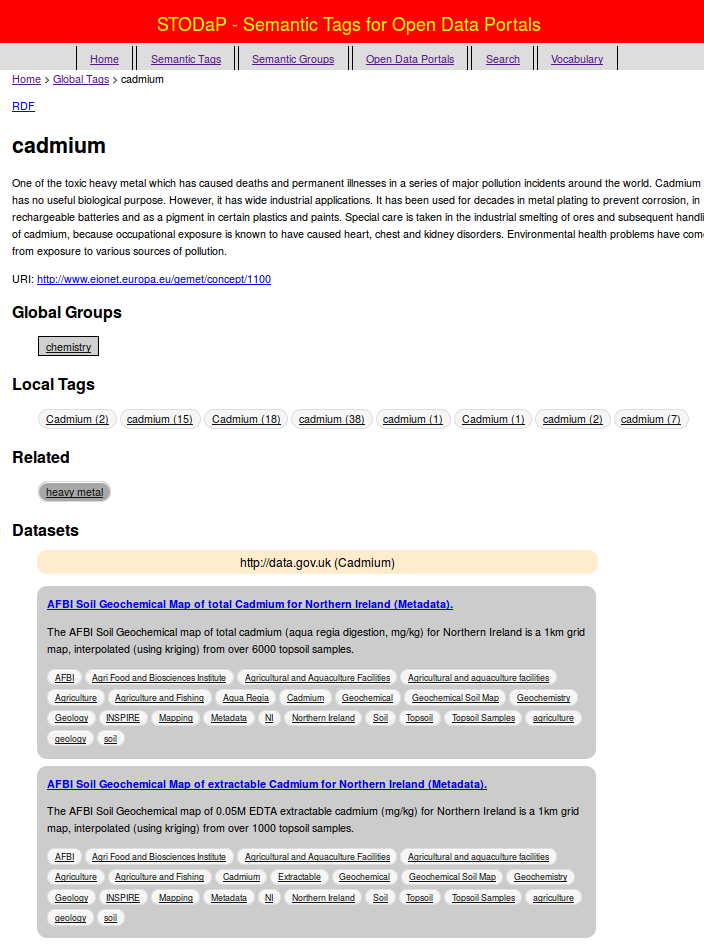
\includegraphics[width=\columnwidth]{images/stodapscreen_semantictag.png}
\caption[Example of the \texttt{cadmium} Semantic Tag.]{Example of the \texttt{cadmium} Semantic Tag. The screen presents a description, the URI, the related Global Groups, Local Tags and Related Datasets}
\label{fig:stodap_semantictag}
\end{center}
\end{figure}

\begin{figure}[h]
\begin{center}
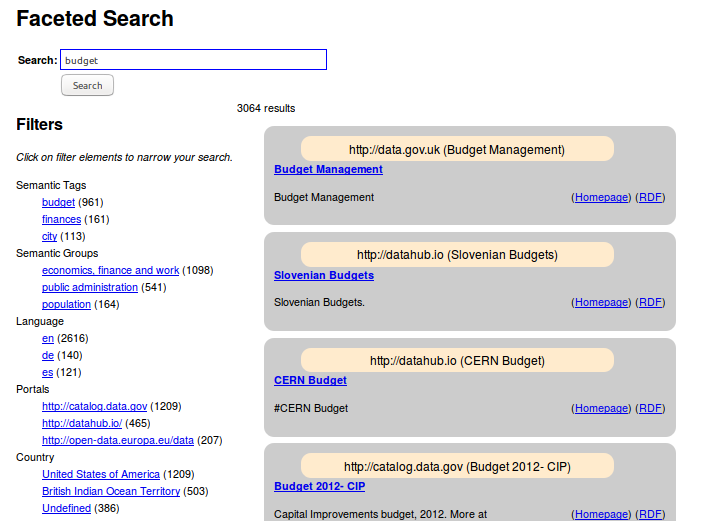
\includegraphics[width=\columnwidth]{images/stodapscreen_search.png}
\caption[STODaP faceted search.]{STODaP faceted search. After inputting a search keyword, facets are presented -- Semantic Tags, Semantig Groups, Country, Language and Portal -- with the number of results in brackets. Users can narrow results by clicking on the facets.}
\label{fig:stodap_search}
\end{center}
\end{figure}

\subsection{CKAN Plugins}
\label{sec:implem_plugins}

CKAN offers an intuitive plugin development environment, which enables developers to modify or extend core functionalities of the system.
The plugin architecture brings advantages both to core maintainers, that can keep their focus on the main functionalities of the platform, and for site managers, who can keep their instances only with desired functionalities.
Plugins can be easily installed by downloading the code and modifying one line at the configuration file.
Communication between plugins and CKAN core is done via CKAN Api\footnote{Available at \url{http://docs.ckan.org/en/latest/api/index.html}.}.
Plugin can also implement logic operations and create new interface templates.

In order to implement tag cleaning and semantic linking functionalities, two plugins were implemented, and their description is in the following:

\noindent\textbf{CKAN Tag Manager Plugin}

The CKAN Tag Manager Plugin offers an environment for tag curation directly inside the CKAN platform. 
It comprises basic functions such as deletion and editing of tags (not present in CKAN core), and advanced function aimed to enhance the quality of tags.
In this sense, the plugin looks for:
\begin{itemize}
	\item Very similar tags, differing only by capitals or special characters;
	\item Similar tags, with a Levenshtein distance $\le 2$ (after lowercasing and unaccenting)
	\item Possible synonyms, using Natural Language Toolkit~\cite{Bird2009} and the WordNet database.
\end{itemize}
In all those cases, user is offered the option of merging the respective pair of tags.
\autoref{fig:local_curation} shows a screenshot of the CKAN Tag Manager.
The plugin was developed using CKAN API in Python language, and can be installed in any CKAN instance. The source code is available for download and contributions at \url{https://github.com/alantygel/ckanext-tagmanager}.


\begin{figure}[h]
\begin{center}
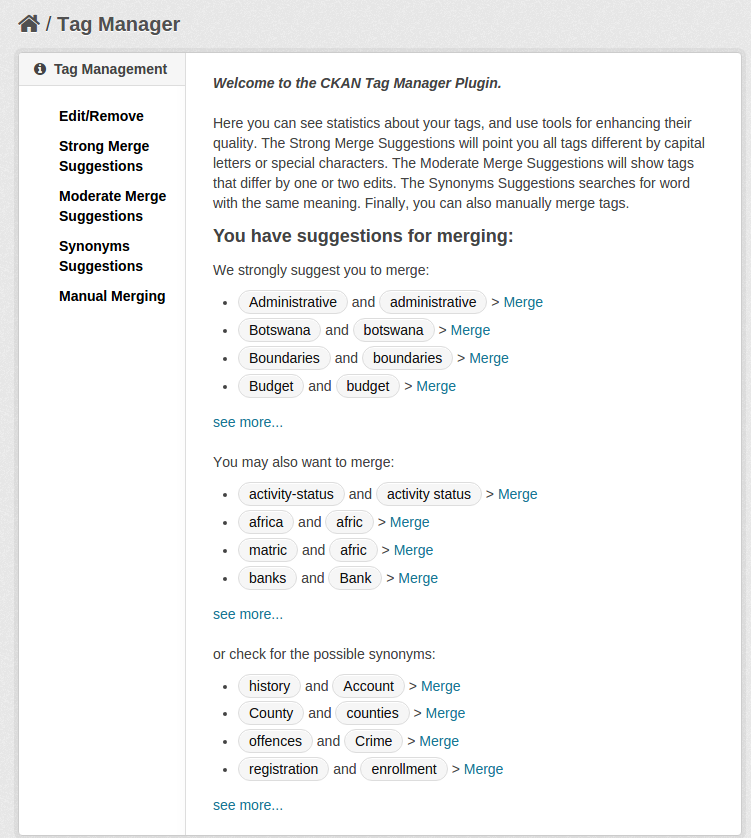
\includegraphics[width=\columnwidth]{images/local_curation.png}
\caption[Screenshot of the Tag Manager plugin.]{Screenshot of the Tag Manager plugin, for tag curation in a CKAN instance. The plugin offers possibilities of manual and semi-automatic tag merging. The first block contains only valid suggestions, while the second block shows 2 false-positives. The synonym module also detected plurals. Tags in this example were extracted from the africaopendata.org portal.}
\label{fig:local_curation}
\end{center}
\end{figure}

\noindent\textbf{CKAN Semantic Tags Plugin}

The CKAN Semantic Tags plugin implements the connection between a CKAN instance and the Semantic Tag Server.
Each local tag can be associated to a semantic tag from the server.
After the association, datasets linked with a local tag also point to the global server, as shown in \autoref{fig:local_link}.

\begin{figure}[ht]
\begin{center}
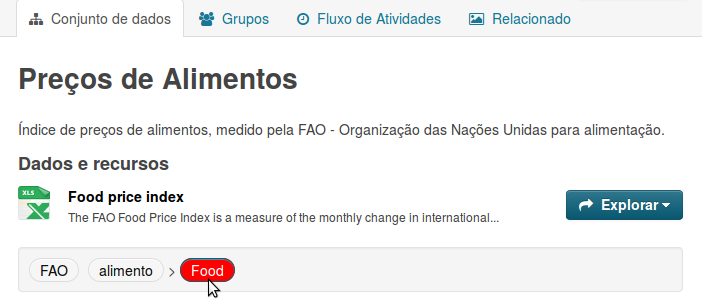
\includegraphics[width=\columnwidth]{images/local_link.png}
\caption[Screenshot of the Semantig Tag plugin.]{Screenshot of the Semantig Tag plugin. The dataset is tagged with two tags, and one of them (\texttt{alimento}) is connected to the semantic tag \texttt{http://stodap.org/tags/Food} through the \texttt{muto:hasTag} property.}
\label{fig:local_link}
\end{center}
\end{figure}

The plugin was developed using CKAN API in Python language, and can be installed in any CKAN instance. The source code is available for download and contributions at \url{https://github.com/alantygel/ckanext-semantictags}.

\subsection{Use and Maintenance of the STODaP server}
\label{sec:use_and_maintenance}

After building the Semantic Tag Server (STODaP), it is necessary to maintain and enhance the tag corpus alongside the evolution of ODPs, as well as to maintain the server updated.
In this subsection, the strategy for it will be presented at the server level.

The first step for building the semantic tag server is to harvest metadata from open data portals.
After the initial setup, a strategy for maintaining the portal up-to-date is needed.

\textbf{Adding a new portal}

When a new ODP is added to the system, a setup procedure is followed:
\begin{itemize}
	\item Harvest tags, datasets and groups metadata;
	\item Clean and group similar tag;
	\item Translate tags, in case of non-English portal;
	\item Reconcile tags with existing Semantic Tags;
	\item If reconciliation is not successful, search lexvo.org and try to create a new semantic tag;
	\item Groups: reconcile with existing global groups or create new ones.
\end{itemize}

\textbf{Updating a portal}

When an ODP is updated, the procedure followed is:
\begin{itemize}
	\item Harvest tags, datasets and groups metadata;
	\item Verify which datasets were inserted or modified
\end{itemize}

%#########################################################################################
\section{Quantitative Results}
\label{sec:results}
%#########################################################################################

We describe in this section some quantitative results achieved with the STODaP approach.
A deeper qualitative evaluation is driven in the next chapter.
At the global level, we analyse some aspects of the implementation.
At the local level it is only possible to claim potential results, as we do not have access to the single ODPs.

\subsection{STODaP Server}

From a total of 291.805 Local Tags, we extracted 2142 Semantic Tags, all linked to the Gemet Thesaurus.
The 1743 Local Groups resulted in 74 Semantic Groups, which are linked to the top concepts of the Gemet Thesaurus.
Between Semantic Tags, we found 3314 relations, being 1355 typed as \texttt{skos:broader}, 1355 as \texttt{skos:narrower} and 604 as \texttt{skos:related}.

% In order to test the system, an open-source implementation of STODaP was created and deployed at \url{http://stodap.org}.
% The following approach was used create 663 semantic tags at the server:
% \begin{itemize}
% 	\item From the 220,567 tags harvested, we selected the 663 that were used in more portals, representing all tags used in 10 or more portals; 
% 	\item Using the Lexvo.org service, we found URI candidates to represent the tag meaning via the \texttt{lexvo:means} property;
% 	\item Using the Lexvo.org service, we found translations and synonyms for the tags via the \texttt{rdf:seeAlso} and \texttt{lexvo:translate} properties;
% 	\item We searched for the translations and synonyms in the harvested tags and included the results as \texttt{muto:taggedResources}, together with the portals tagged with the original term;
% 	\item Using the \href{http://www.nltk.org/}{Natural Language Toolkit  Library}, we searched for semantic similar semantic tags, which were added as \texttt{skos:related}.
% \end{itemize}

% The occurrence of the original tags among the portals, and the results after including the translations and synonyms can be seen in \autoref{fig:results_tagged_resources}. 
% The graphic shows the 30 most used tags, and the achieved increment in the number of relations. 
% The occurrence of tags denoting years can also be noticed.
% Obviously these tags have no synonyms nor translations, and thus no increment is shown. 
% It is also worth mentioning that the tag \texttt{{test}} is the fourth most used one.
% This fact is probably related to the early stage of development of some portals. 

% \begin{figure}[tb]
% \begin{center}
% 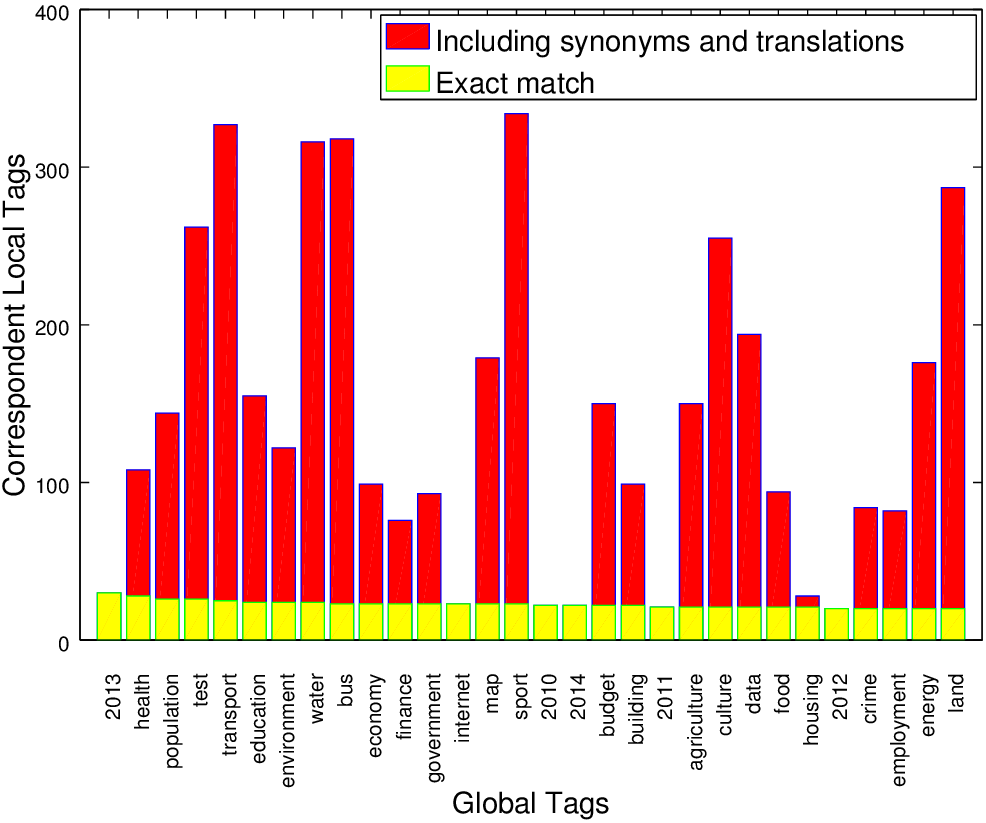
\includegraphics[width=\columnwidth]{images/results_tagged_resources.png}
% \caption[Correspondence between local and semantic tags.]{Correspondence between local and semantic tags. The yellow bar shows the number of exact occurrences of the tag in ODPs. The red bar shows the improvement when considered translations and synonyms, which can also occur in a same portal. This explains the numbers over 90. }
% \label{fig:results_tagged_resources}
% \end{center}
% \end{figure}

\subsection{Local Level}

At the local level, the main potential achievements are at the tag curation process.
As shown in \autoref{fig:similarity}, a considerable number of pairs of tags differ only by capital or accented characters.
Using the naive approach to merge similar tags in every portal would result in reducing the number of 14,168 local tags, which represents 6.4\% of the total number of tags.
Lowercase and unaccented tags differing by a Levenshtein-distance from 0 to 2 represent a total of 35,066 pairs, or 15,8\% from the whole tag universe.
However, as discussed above, this approach can lead to false-positives and thus requires manual checking.


\section{Our Contribution Regarding the State of the Art}
% talvez puxar para o final do capitulo 5

In this chapter, we presented the state of the art in each of the steps for dealing with the problem of semantic organization of ODPs.
In relation to the cited works, we are advancing on this field in the following aspects:
\begin{itemize}
	\item Instead of dealing with folksonomies, i.e., several users tagging the same resources in the same platform, our problem is related to few administrators tagging different resources on different platforms.
	\item Our approach is multi-language;
	\item We implemented a platform for semantically linking datasets through semantic tags;
	\item Dealing with the context of ODPs.
\end{itemize}

Offline: \citeonline{Marchetti2007}
\cite{Passant2008}

%#########################################################################################
\section{Conclusions}
\label{sec:stodap_conclusions}
%#########################################################################################

In this chapter, we presented an approach for metadata reconciliation within and among Open Data Portals.
The main objective of this approach is to tackle the open data organization problem, which was shown to be a relevant in the previous chapters.
In \autoref{chap:dataliteracy}, one of the results of a participatory research based on Data Literacy courses pointed out to the difficulties of novice users in finding open datasets.
A literature based research in \autoref{chap:opendata} and \autoref{chap:relworks} also pointed to the organization problem as relevant to the development of open data.
On the analysis driven in previous chapter, we found that several portals share the same tags, showing that tags have a good potential to be linking elements among datasets.
Converting tags into semantic identifiers was also shown as a viable option, even though more sophisticated methods have to be investigated. 
Based on these findings, we derived the STODaP approach, which comprises two parts: 
a local one, aimed at cleaning up and enhancing the quality of ODPs tags, and 
a global one, for connecting ODPs through semantic tags.
The implementation of both shows that significant enhancements can be achieved both at the individual ODPs and the global levels.
In the next chapter, an evaluation of this approach is presented.


%1) juntar grupos 
%2) ver quantas tags e datasets estão la dentro
%3) dentro de cada grupo organizar melhor

%Categorization: http://eurovoc.europa.eu/drupal/?q=navigation&cl=en
%Categorization: http://www.eionet.europa.eu/gemet/

